\chapter{State-of-the-Art Verfahren zur semantischen Segmentierung von 3D-Daten}
\section{PointNet}
PointNet ist eine fortschrittliches Methode zur Verarbeitung von Punktwolken in
der 3D-Bild-verarbeitung, die speziell für die Aufgaben der Klassifikation,
Segmentierung und Erkennung von Objekten entwickelt wurde. Das Verfahren
arbeitet dabei direkt auf den Punktwolken-Daten, ohne diese in ein Voxelgitter
oder eine andere Form zu überführen. Dadurch wird eine höhere Genauigkeit und
Effizienz erreicht. Zu Beginn des Netzwerkes wird das sogenannte T-Net
(Transformations-Netzwerk) auf den Datensatz angewendet. Dadurch wird dieser in
eine kanonische Form übergeführt, welche invariant gegenüber Transformationen
und Skalierungen von Strukturen ist. Die Kernkomponente der PointNet-Architektur besteht in
der Unterteilung des Netzes in ein Klassifikations- und ein
Segmentierungsnetzwerk. Der Klassifizierungsteil extrahiert dabei globale
Merkmale des Eingangsbildes. Der Segmentierungsteil verwendet dann sowohl
lokale, als auch globale Merkmale, um die Segmentierung der Punktwolke
durchzuführen. Durch die Kombination beider Netzwerke lässt sich eine höhere
Robustheit und Genauigkeit erreichen. Der Aufbau von PointNet ist schematisch
in Abbildung \ref{fig:pointnet} dargestellt. \cite{8099499} Eine bekannte
Erweiterung von PointNet ist PointNet++. Dieses Verfahren unterscheidet sich
durch eine hierachische Struktur, wodurch globale und lokale Merkmale besser
erfasst werden können. \cite{NIPS2017_d8bf84be}

\begin{figure}[h]
    \centering
    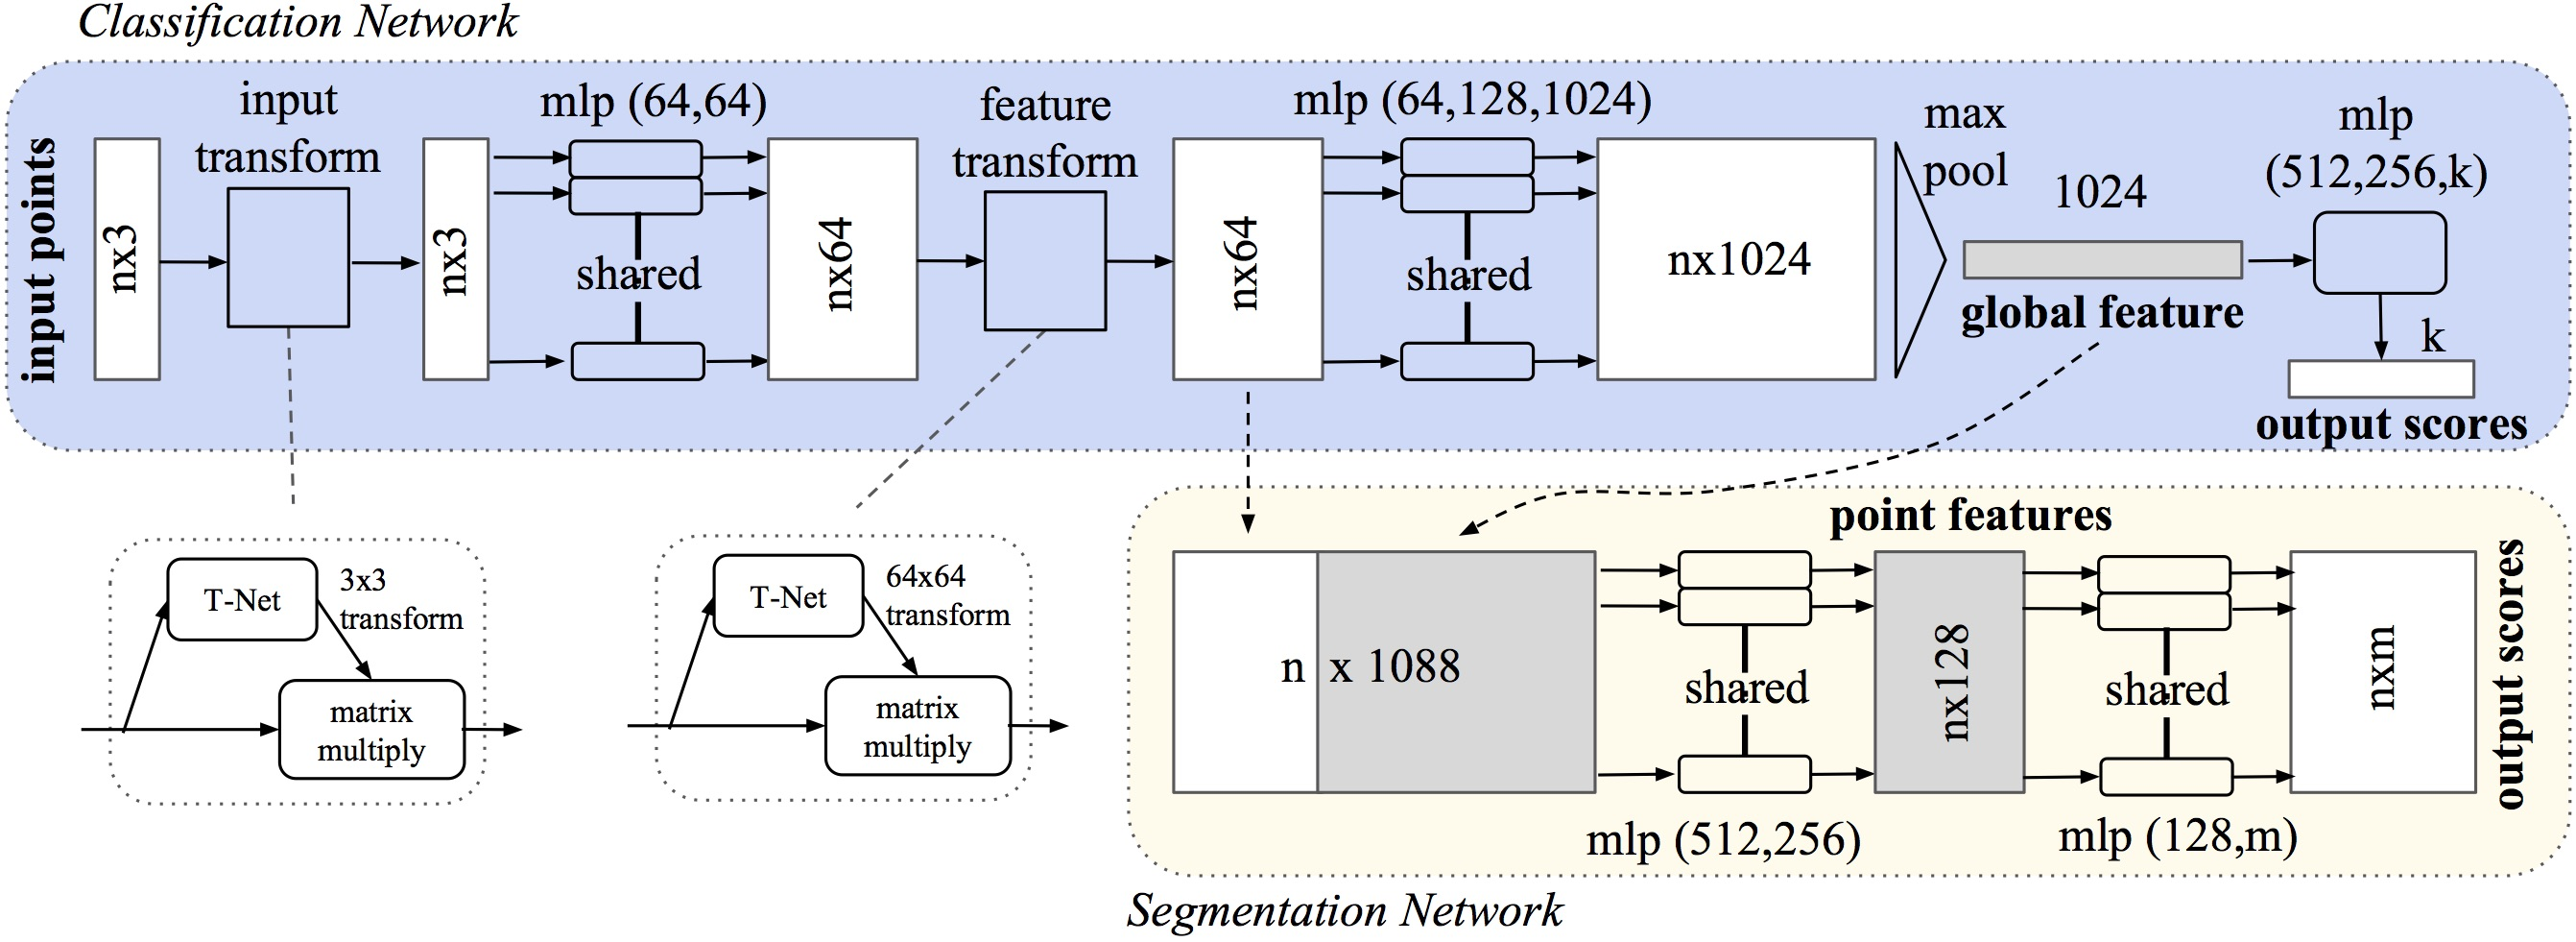
\includegraphics[width=0.8\textwidth]{bilder/pointnet.jpg}
    \captionsetup{font=small} % Hier die gewünschte Größe einstellen

    \caption[PointNet-Architektur]{PointNet-Architektur \cite{8099499}}
    \label{fig:pointnet}
\end{figure}

\section{3D U-Net}

3D U-Net ist ein leistungsstarkes Verfahren für die semantische Segmentierung von 3D-Daten.
Es basiert auf der verbreiteten 2D U-Net-Architektur, die für die Bildsegmentierung entwickelt wurde \cite{ronneberger2015unet}.
Um diese Architektur auf 3D-Daten anzuwenden, wurde sie entsprechend angepasst.
Die 3D U-Net-Architektur besteht aus einem Encoder-Decoder-Netzwerk mit
Skip-Connections. Der Encoder-Teil nimmt das Eingabevolumen entgegen und
besteht aus mehreren Convolutional-Layers, gefolgt von Pooling-Layern. Diese
Schichten helfen dabei, wichtige Merkmale des Eingangsbildes zu extrahieren und
die räumliche Auflösung zu reduzieren. Die Skip Connections werden zwischen den
Encoder- und Decoder-Schichten erstellt, um beim Prozess des upsamplings eine
positionsgetreue Wiederherstellung der Bildmerkmale zu gewährleisten. Der
Decoder-Teil des 3D U-Net-Netzwerks besteht dabei aus Upsampling-Schichten, die
die räumliche Auflösung erhöhen, gefolgt von Deconvolutional-Layers. Der Name
des Netzes leitet sich dabei aus dessen Architektur ab, welche in Abbildung
\ref{fig:UNET} dargestellt ist. 
Ein wesentliches Merkmal von 3D U-Net ist dessen Fähigkeit, volumetrische
Kontextinformationen zu berücksichtigen. Durch die Verarbeitung von
3D-Volumendaten können komplexe räumliche Zusammenhänge erfasst und genutzt
werden, um eine präzise Segmentierung zu erreichen. Das Verfahren findet insbesondere in
medizinischen Bereichen Anwendung, in denen die genaue Abgrenzung
von Organen oder Tumoren entscheidend ist. \cite{cciccek20163d,987654321}\\

\begin{figure}[H]
    \centering
    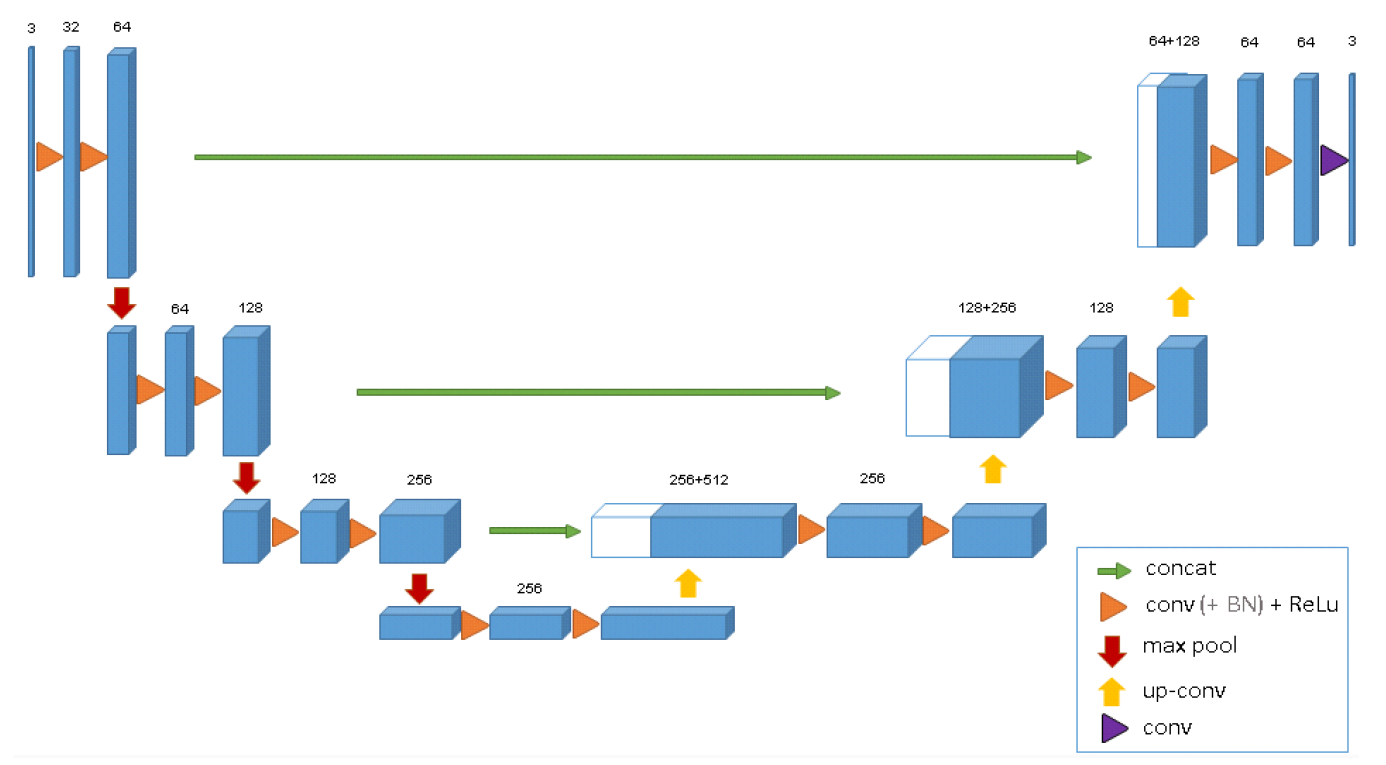
\includegraphics[width=0.8\textwidth]{bilder/3D_U-Net.png}
    \captionsetup{font=small} % Hier die gewünschte Größe einstellen

    \caption[3D U-Net Architektur]{3D U-Net Architektur \cite{cciccek20163d}}
    \label{fig:UNET}
\end{figure}